\section{Related Work}
\label{sec:related_work}

% Test case generation from natural-language documents has evolved along three paradigms, model-based, LLM-based, and hybrid, as illustrated in Figure~\ref{fig:related_work}. We review these paradigms and their application to regulatory compliance testing.

\subsection{Test Generation from Natural-Language Requirements}

Test generation from natural-language requirements follows three broad paradigms. \textit{Model-based methods} derive tests from explicit behavioral or structural representations, including control-flow graphs~\cite{yang2025llmcfg}, system graphs~\cite{zyberaj2025genai}, Operational Design Domain models~\cite{stefani2025automated}, and domain-specific models for financial systems~\cite{jin2019finexpert}. These representations support systematic generation and inspection, but creating or adapting them often requires domain-specific modeling effort~\cite{xue2024domain}.

\textit{LLM-based methods} generate test specifications directly from requirements through prompt engineering and prompt chaining~\cite{masuda2026generating,bhatia2024system,boukhlif2024towards}, or decompose the task into multiple generation stages~\cite{milchevski2025multi}. Comparative and industrial studies report improved automation but also expose sensitivity to prompts, models, and requirement complexity~\cite{hasan2025automatic,korraprolu2025test,wang2025testeval,zhang2024testbench}.

\textit{Hybrid methods} combine LLMs with explicit domain artifacts. Examples include domain-model-guided financial acceptance testing~\cite{xue2024llm4fin}, ontology-guided BIM compliance checking~\cite{chen2024automated}, retrieval-grounded compliance checking~\cite{sun2025compliance}, and test generation from formal requirements~\cite{shrestha2025less}. These artifacts improve structure and controllability, but when they are manually engineered, adaptation shifts effort from test generation to knowledge construction and maintenance.


% Model-based approaches derive test cases from intermediate behavioral or structural models, such as graphs, domain models, and formal specifications, via techniques like graph traversal, symbolic execution, and constraint solving. For instance, Yang et al. construct Control Flow Graphs (CFGs) from requirements and enumerate executable paths~\cite{yang2025llmcfg}, Zyberaj et al. transform specifications into System Graphs (SGs) for test generation~\cite{zyberaj2025genai}, and in safety-critical domains, Operational Design Domain (ODD) models and formal representations are used to capture regulatory constraints for testing~\cite{stefani2025automated,jin2019finexpert}. Such explicit modeling offers strong interpretability and controllability, but building and maintaining the models demands substantial expertise, raising cost and limiting portability across domains~\cite{xue2024domain}.


% Model-based approaches generate test cases by first transforming the rules or requirements into intermediate models, such as graphs, domain models, or formal representations, and then applying algorithmic analysis such as traversal and constraint solving.
% For example, Yang et al. construct Control Flow Graphs (CFG) from requirements and generate test cases by enumerating executable paths \cite{yang2025llmcfg}.
% Zyberaj et al. convert system specifications into structured System Graphs (SG), from which executable scenarios are derived to support efficient test case generation \cite{zyberaj2025genai}.
% In safety-critical domains, researchers further employ domain-specific models, such as Operational Design Domain (ODD) models and Formal Representations (FR), to encode regulatory knowledge, constraints, and requirements, and to support subsequent compliance test case generation \cite{stefani2025automated,jin2019finexpert}.

% While model-based approaches offer strong controllability and interpretability, they rely on manual or rule-based NLP tools to construct intermediate models. Building and maintaining such models requires substantial domain expertise and engineering effort, thereby limiting scalability in real-world settings \cite{xue2024domain}.



% \vspace{1mm}
% \noindent
% \textbf{LLM-Based Test Generation.}
% LLM-based methods generate test cases from natural-language requirements, specifications, or regulations using LLMs. Prompt-based methods guide LLMs via prompt engineering or chaining, e.g., extracting test design techniques before generation~\cite{masuda2025generating} or chaining prompts to produce structured test artifacts~\cite{bhatia2024system}. Agent-based methods decompose generation into coordinated stages to simulate professional testing workflows~\cite{milchevski2025multi} or stress testing and diagnosis~\cite{jin2025guard}. Domain adaptation via RAG, supervised fine-tuning (SFT), and reinforcement learning (RL) has also been explored~\cite{boukhlif2024towards,hasan2025automatic}. These methods improve automation and flexibility, yet LLM stochasticity leaves them prone to hallucinations and inconsistent outputs, limiting reliability in safety-critical compliance testing~\cite{wang2025testeval,korraprolu2025test,zhang2024testbench}.


% LLM-based approaches generate test cases directly from natural language requirements, either via prompt engineering or agent frameworks.

% Prompt-based approaches rely on prompt engineering to guide LLMs in test generation. Masuda et al. extract test design techniques before generating high-level test cases~\cite{masuda2025generating}. 
% Bhatia et al. employ prompt chaining to produce structured test tables from full documents~\cite{bhatia2024system}. 
% Despite their simplicity and flexibility, these methods suffer from limited reliability: they struggle to target specific execution branches and degrade on complex requirements due to insufficient reasoning and lack of domain knowledge~\cite{wang2025testeval,korraprolu2025test}.

% Agent-based systems address these limitations by decomposing test generation into coordinated stages. 
% Milchevski et al. design a multi-agent framework that simulates professional testing workflows, including requirements analysis, test design, and generation~\cite{milchevski2025multi}. 
% Jin et al. adopt multi-LLM orchestration for stress testing and diagnostic analysis~\cite{jin2025guard}. 
% While RAG and fine-tuning have been explored for domain integration ~\cite{boukhlif2024towards,hasan2025automatic}, these approaches remain limited by LLM stochasticity, leading to hallucinations, unstable outputs, and incomplete coverage of critical program behaviors\cite{zhang2024testbench,korraprolu2025test}.

% \vspace{1mm}
% \noindent
% \textbf{Hybrid Frameworks.}
% Hybrid approaches guide LLMs with domain knowledge artifacts, such as ontologies, schemas, templates, or formal specifications, to construct intermediate representations that support test generation. For example, Xue et al. use a domain meta-model to guide LLM-based information extraction and combine it with scenario synthesis for financial compliance testing~\cite{xue2024llm4fin}, Chen et al. embed domain ontologies into an LLM-assisted pipeline for compliance checking in BIM~\cite{chen2024automated}, and others apply requirement templates or formal schemas to constrain generation~\cite{sun2025compliance,shrestha2025less}. Such grounding improves reliability and controllability, but the artifacts are typically hand-engineered and costly to maintain when adapting to new regulations or domains, shifting the bottleneck from test generation to knowledge engineering.


% Hybrid approaches aim to bridge the gap between the above two methods by using LLMs to construct intermediate models, guided and constrained by domain knowledge such as ontologies, schemas, or formal specifications. These intermediate models are then leveraged for test generation.
% For example, Xue et al. define a domain meta-model to guide LLM-based information extraction and integrate it with rule-driven scenario synthesis, enabling automated test case generation from business rules~\cite{xue2024llm4fin}.
% Chen et al. incorporate domain ontologies into an LLM-assisted pipeline for compliance checking in BIM, enabling more precise interpretation of regulatory texts \cite{chen2024automated}.
% Other approaches adopt RAG or requirement templates to further constrain LLM outputs~\cite{sun2025compliance,shrestha2025less}.

% Although grounding LLM generation in domain knowledge mitigates hallucinations, manual knowledge construction limits scalability and adaptability, necessitating automated methods that reduce human involvement and enable generalizable test generation.



\subsection{Regulatory Compliance Testing}
Compliance testing has attracted growing attention in regulated settings. Earlier work formalizes regulations using controlled natural language, knowledge representations, and SBVR models~\cite{roychoudhury2018case,kholkar2016natural,roychoudhury2017natural}. More recent systems address financial acceptance-test generation with domain models~\cite{xue2024llm4fin}, retrieval-grounded regulatory compliance checking~\cite{sun2025compliance}, and formal-requirement-guided test generation~\cite{shrestha2025less}; adjacent industrial work assesses software adherence to automotive safety standards~\cite{tabani2019assessing}. These studies address different downstream tasks but commonly depend on domain-specific regulatory artifacts. \ourtool\ instead automates reusable meta-level artifact construction while keeping regulatory text authoritative.





\subsection{Knowledge Extraction from LLMs}
A growing body of work treats LLMs as queryable knowledge sources. Petroni et al.~\cite{petroni2019language} showed with the LAMA probe that pre-trained models can recall factual knowledge without fine-tuning. Subsequent probing- and prompting-based methods extract factual triples~\cite{jiang2020can,alivanistos2022prompting} or construct knowledge graphs at scale~\cite{bian2025llm}, although the extracted knowledge is often sensitive to prompt design and difficult to verify~\cite{youssef2023give}. These methods primarily target generic knowledge represented as triples or general-purpose graphs, whereas compliance testing requires domain-specific conceptual, representational, and testability artifacts. \ourtool\ therefore constructs candidate meta-level artifacts with multiple LLMs and consolidates them through artifact-specific purification or aggregation.

\begin{figure*}[!t]
    \centering
    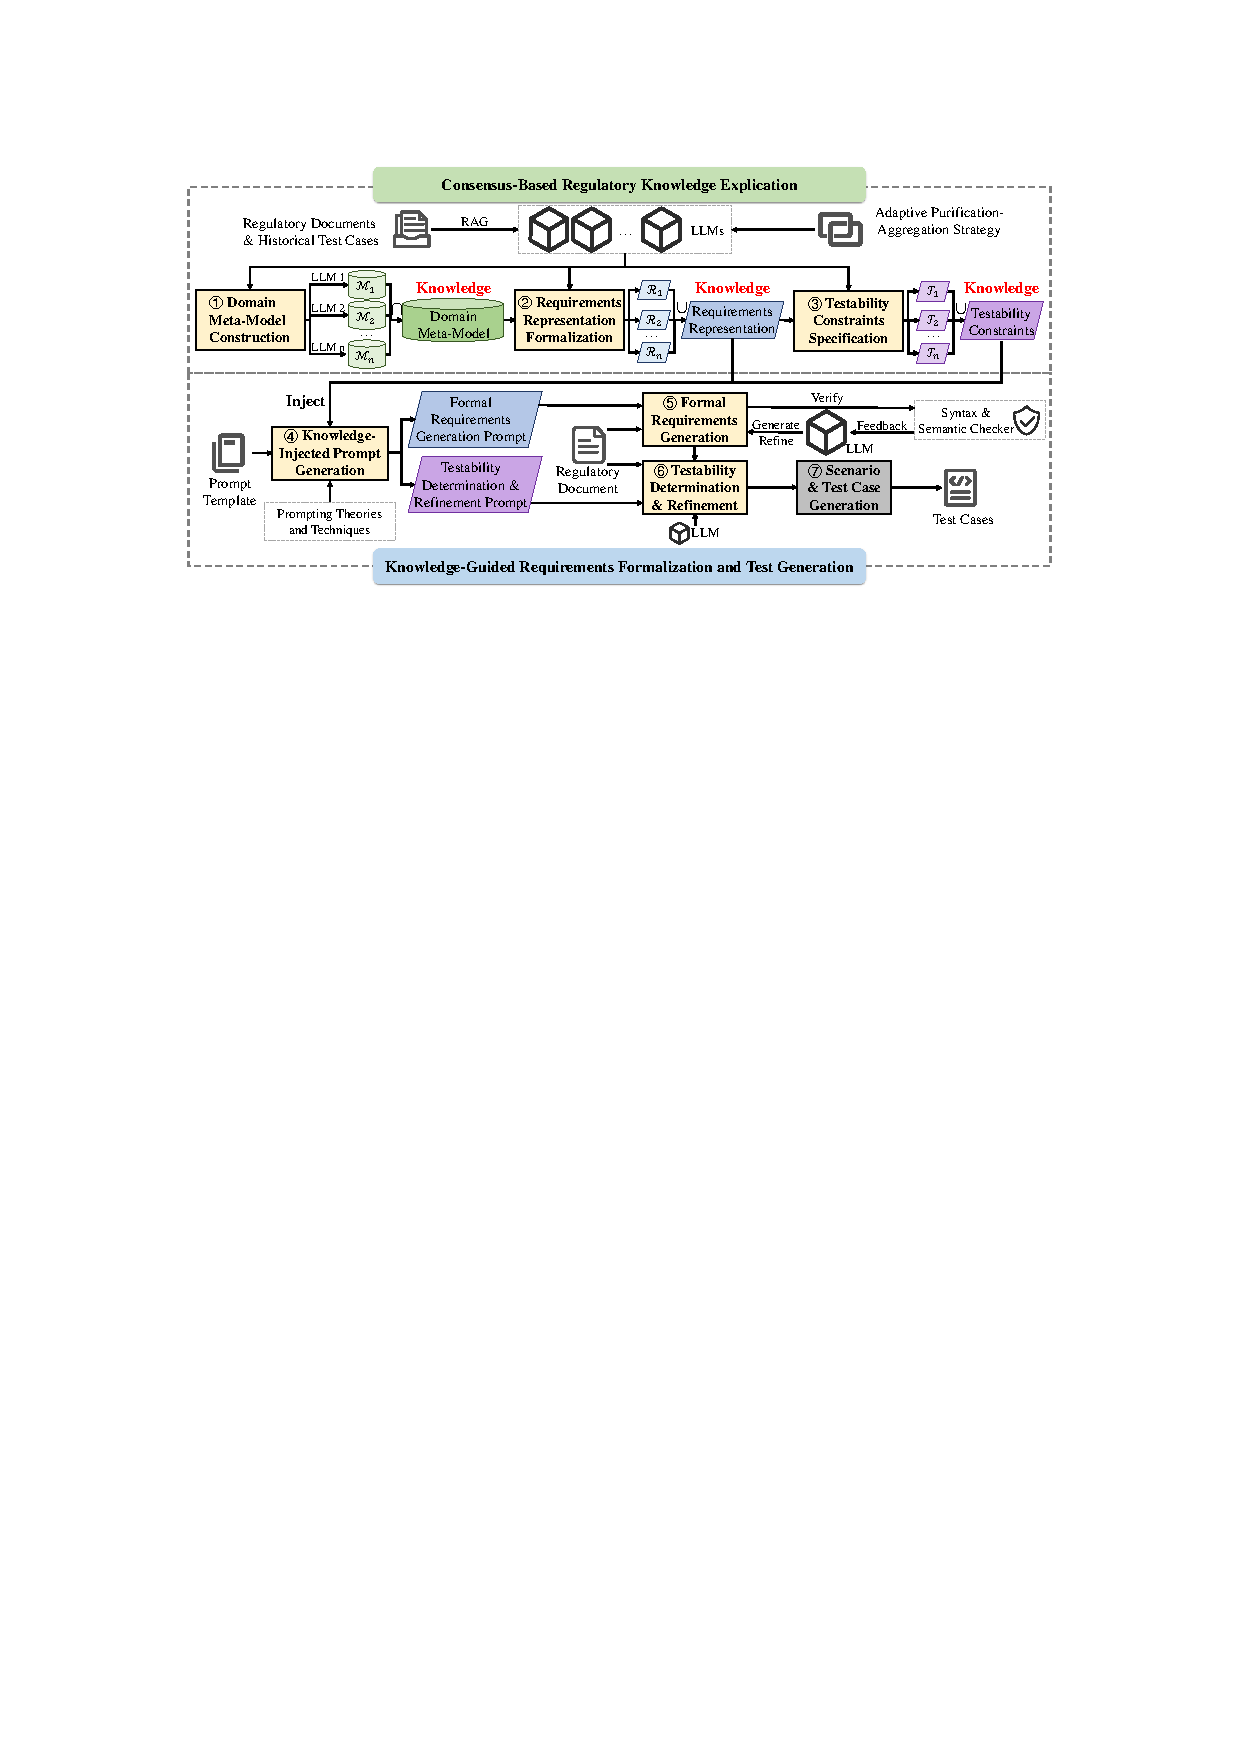
\includegraphics[width=0.9\linewidth]{fig/framework.pdf}
    \caption{\ourtool's knowledge-explication and knowledge-injected test-generation workflow.}
    \label{fig:framework}
    \Description{The RAFT workflow first explicates a domain meta-model, requirements representation, and testability constraints, then injects them into requirements formalization, testability refinement, and test generation.}
\end{figure*}
